\chapter{Wavelets theory}
A ''wavelet'' literally means a small wave. This term says a lot about its nature. Wavelets are a family of functions which oscillates like wave and should be compactly supported. Additionally, the wavelet has zero mean.

\begin{defn}
Wavelets are created by scaling and shifting of the, so called, mother wavelet $\psi(t)$. The child wavelets are defined as

\begin{equation}
\label{eq:wavelets}
\psi^{(a,b)}(t)=|a|^{-\frac{1}{2}} \psi\left(\frac{t-b}{a}\right),\ a>0,
\end{equation}

where $a$ is a scale parameter and $b$ translation parameter.

\end{defn}

There are plenty of different mother wavelets, for example

\begin{figure}[h]
	\centering
	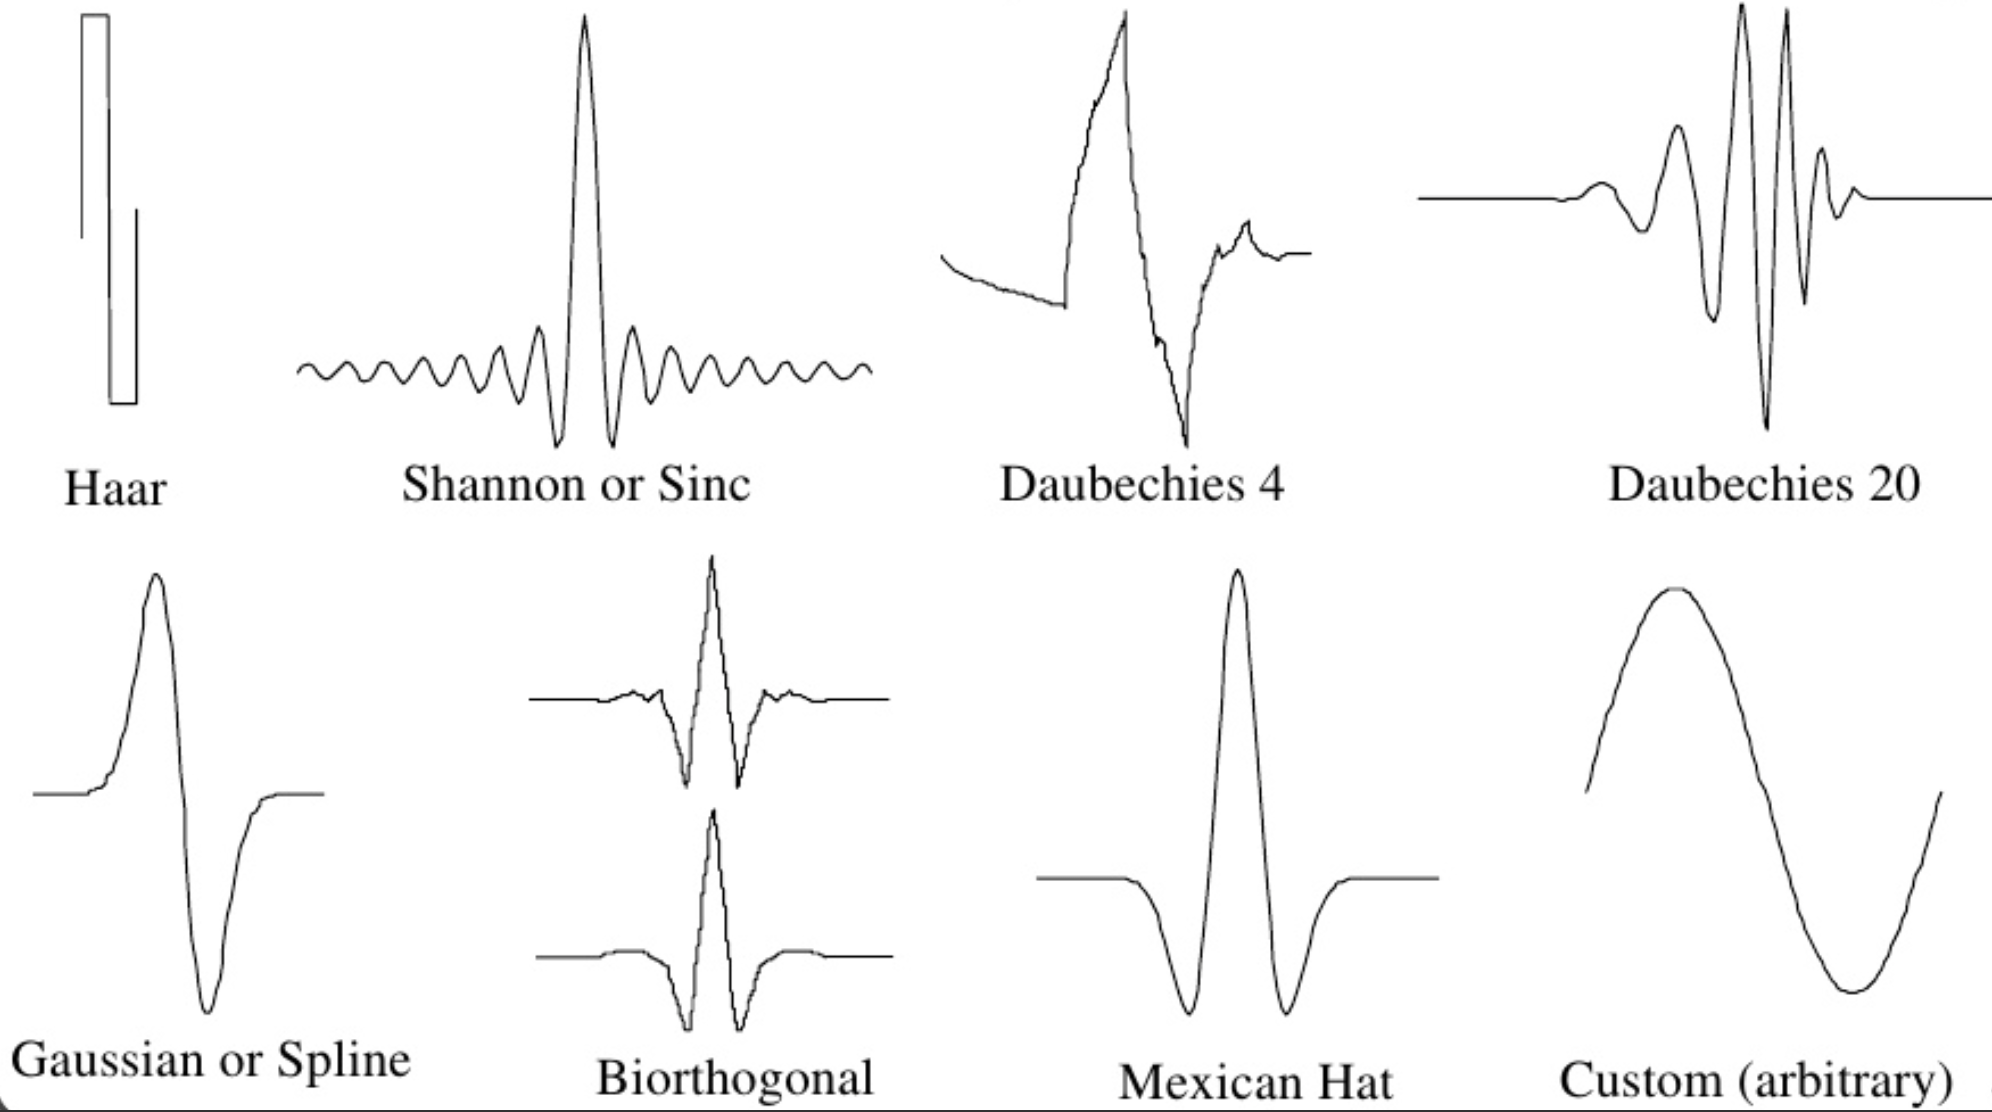
\includegraphics[width=\textwidth]{wavelets_with_bottom_line.png}
	\caption{Different types of wavelets.}
	\label{fig:wavelets}
\end{figure}

\textit{** I'll add more about wavelets properties - orthogonal basis, decorrelated coefficients, vanishing moments, compact support. And how those properties can be useful in data mining. **}


\section{Haar and Daubechies wavelets}

\textit{** Add that db1 is the same as Haar. Add little more about specific properties for this wavelet family. **}

Each type of wavelet function is more suitable for different applications. The best for image analysis are the Daubechies wavelets. 

\begin{defn}
Daubechies wavelets are collection of orthogonal and compactly supported functions. A denotation for those wavelets is $dbN$, where $N$ means a maximal number of vanishing moments.
\end{defn}

\begin{figure}[h]
	\centering
	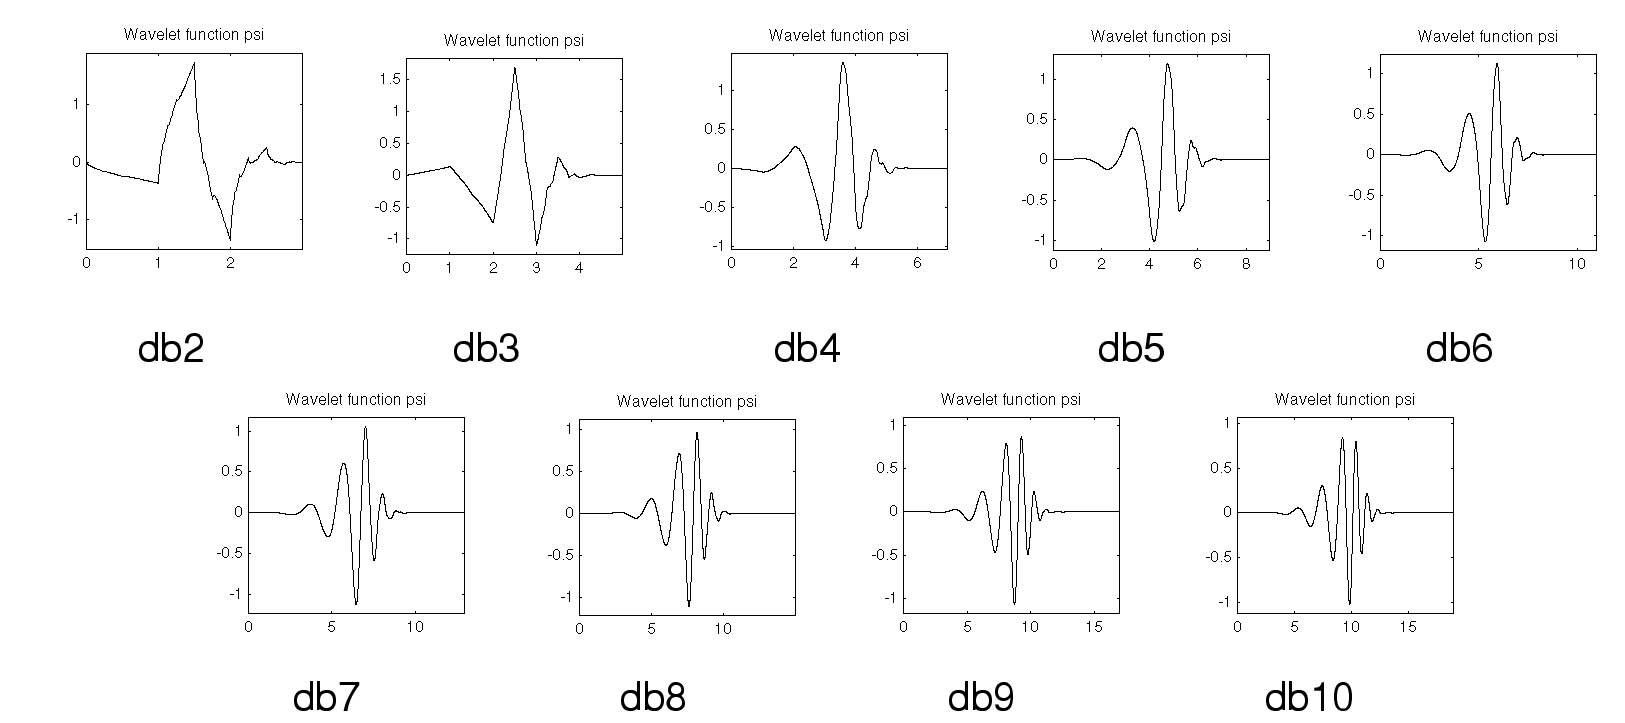
\includegraphics[width=\textwidth]{DB_N.png}
	\caption{Daubechies wavelets.}
	\label{fig:db_wavelets}
\end{figure}

\section{Wavelet Transform}

Generally, integral transforms are useful in data processing. Their idea is to convert data into another domain, where it is easier to manipulate them, finding desired informations, etc. Finally, the results are transformed back to the original domain by inverse integral transform.

We can define integral transform based on the wavelet functions - Wavelet Transform.
However, the most popular kind of integral transform is Fourier Transform. Here the question arises, what are the differences between both operators. Lets start from the definitions.

\begin{defn}
Continuous Wavelet Transform is expressed by the formula

\begin{equation}
W(a,b)=\int_{-\infty}^{\infty} y(t) a^{-\frac{1}{2}} \psi\left(\frac{t-b}{a}\right) dt,
\end{equation}

where $a$ is scale parameter, $b$ translation parameter and $y(t)$ original signal.
\end{defn}


\begin{defn}
Fourier transform is defined as

\begin{equation}
Y(f)=\int_{-\infty}^{\infty} y(t) e^{-i\omega t} dt,
\end{equation}

where $y(t)$ is time domain signal and $Y(f)$ is frequency domain signal.
\end{defn}

The most important differences are presented in the table below.

\begin{table}[h]
\centering
\begin{tabular}{|p{0.5\linewidth}|p{0.5\linewidth}|}
\toprule
\textbf{ Wavelet transform} & \textbf{Fourier transform}
\\ \midrule
Suitable for stationary and non-\allowbreak -stationary signals 
& Suitable for stationary signals 
\\ \midrule
High time and frequency resolution
& Zero time resolution and very high frequency resolution     
\\ \midrule
Very suitable for studying the local behaviours of the signal
& No suitable  
\\ \midrule
Scaled and translated mother wavelets
& Sine and cosine waves
\\ \bottomrule
\end{tabular}
%\label{tab:wt_vs_ft}
\caption{The comparison of Wavelet and Fourier Transform.}
\end{table}

The obvious distinction between both transforms is the type of function. In Fourier case there are sine and cosine functions, wherein wavelet transform uses wavelets. Sine function oscillates on the whole real axis, thus it cannot represent abrupt changes. However, the Wavelet transform is localized in space and time, so it can be used to detect trends or sudden changes in signals and images. Moreover, wide range of wavelet functions is a main advantage of wavelet analysis, because we can adjust the type of wavelet to the specific case and thank to that obtain more accurate results.

\section{Discrete Wavelet transform}

There are two types of Wavelet Transform:
\begin{itemize}
	\item Continuous Wavelet Transform (CWT),
	\item Discrete Wavelet Transform (DWT).
\end{itemize}

The Discrete Wavelet Transform has a wide range of applications in image processing, for example denoising and compressing, also in detecting shapes on images.

\textit{** I'll add a little more about applications in pre-processing and machine learning **}

Scale and translation parameters are defined as

\begin{equation}
a = 2^j \text{ and } b = 2^j m,\ j,m=1,2,\ldots.
\end{equation}

Therefore, assuming that $0 \leq t < 2^K$, $K \in \mathbb{Z}$, the coefficients of Discrete Wavelet Transform are defined as follow

\begin{equation}
d^{(j,m)}=\sum_{t=0}^{2^K -1} y(t) 2^{-\frac{j}{2}} \psi\left(2^{-j}t - m\right).
\end{equation}

The figure \ref{fig:DWT} on a page \pageref{fig:DWT} shows how DWT works. Discrete Wavelet Transform splits signal with two filters: $g(n)$ - low pass filter (LPF) and $h(n)$ - high pass filter (HPF). The LPF captures a part with lower frequencies which refers to the main signal. Whereas, the HPF captures higher frequencies - a noise of the signal. Subsequently, both parts are downsampled by a factor of 2. This decomposition can be repeated on the LPF part of the signal. Hence, the next levels of DWT coefficients.

\begin{figure}[h]
	\centering
	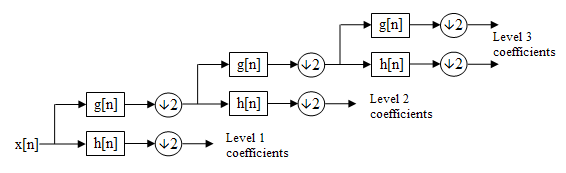
\includegraphics[width=\textwidth]{DWT.png}
	\caption{Discrete Wavelet transform on a signal $x(n)$.}
	\label{fig:DWT}
\end{figure}


\section{2-D Discrete Wavelet transform}
\label{sec:2D_DWT}

2-Dimensional Discrete Wavelet Transform works similar way as 1-D with High Pass Filter, Low Pass Filter and downsampling, except that one level of the decomposition includes double filtering, on columns and rows. The figure \ref{fig:2D_DWT} shows an image decomposition. Firstly, the DWT is applied on columns of the input image and then on the rows of the both outputs. Ultimately, there are four results:

\begin{itemize}
\item LL - result of LPF applied on both, columns and rows,
\item LH - result of LPF applied on columns and HPF on rows,
\item HL - result of HPF applied on columns and LPF on rows,
\item HH - result of HPF applied on both, columns and rows.
\end{itemize}  

\begin{figure}[h]
	\centering
	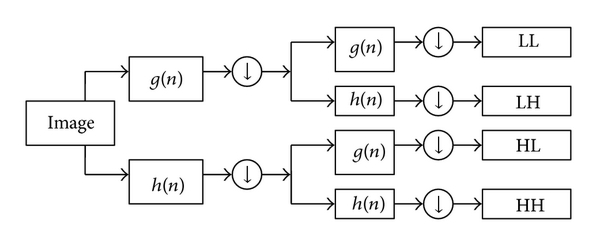
\includegraphics[width=\textwidth]{2D_DWT.JPG}
	\caption{2-D Discrete Wavelet transform on an image.}
	\label{fig:2D_DWT}
\end{figure}

Recall that the outcome of Low Pass Filter in the previous case was the main signal (without a noise). Thus, a 2-Dimensional equivalent is an approximation of an analysed image. The High Pass Filter captures high frequencies, then for an image the outcome are sudden changes in the image contrast. Now, lets focus on what exactly each result represent. First one, the LL is just an approximation of the initial image. Next, the LH shows abrupt changes in a horizontal direction, whereas the HL part presents similar issues but in a vertical direction. The HH shows sudden changes in a diagonal direction. In conclusion, the output of 2-D DWT gives us an approximation of the image and three parts with abrupt changes in different directions.

\section{Inverse Wavelet Transform}

Majority applications of Wavelet Transform assume that data is converted to wavelet domain and ten we can get the desired information. Although, we must return to the original domain for the information to be useful. The Inverse Wavelet Transform allows for such operation.

\begin{defn}
Inverse Discrete Wavelet Transform is defined as

\begin{equation}
y(t) = \sum_{j=1}^{K} \sum_{m=0}^{2^{K-j}-1} d^{(j,m)} 2^{-\frac{j}{2}} \psi\left(2^{-j}t - m\right) + \psi_0,
\end{equation}

where $y(t)$ is reconstruction of the input data and $d^{(j,m)}$ coefficients of wavelet transform. The $\psi_0$ is an average value of $y(t)$ over $t \in [0, 2^K-1]$. This parameter can be approximated by zero, without loss of generality.
\end{defn}

Thus, now we are able to transform data to a wavelet domain, process them simply and efficiently. As well as, we can back to the original domain to read the obtained results.
